\documentclass[a4paper,12pt]{exam}
\usepackage{array,amsmath,fancybox,amsfonts,bm}
\usepackage{graphicx,amssymb,wasysym,latexsym,slashed,anysize,subfigure,calc}



%versores: %uso: \uveci\ne\hat{\imath}_{\uvec{i}}+\uvec{j}+\uvec{k}$
	\usepackage{bm}
	\newcommand{\uveci}{{\bm{\hat{\textnormal{\bfseries\i}}}}}
	\newcommand{\uvecj}{{\bm{\hat{\textnormal{\bfseries\j}}}}}
	\DeclareRobustCommand{\uvec}[1]{{%
 	 \ifcsname uvec#1\endcsname
  	   \csname uvec#1\endcsname
  	 \else
   		 \bm{\hat{\mathbf{#1}}}%
   		\fi
									}}


\usepackage{enumitem}
\setenumerate{itemsep=15pt}

%tamaños fuentes extra: 8,9,14,17,20
	\usepackage{extsizes}
	
 %caja bonita
  \usepackage[many]{tcolorbox}
\definecolor{titlebg}{RGB}{80,100,72}
\newtcolorbox{learn}{
  breakable,
  enhanced,
  arc=0pt,
  outer arc=0pt,
  colframe=titlebg,
  colback=titlebg!7,
  overlay unbroken and first={
    \node[
      draw=titlebg,
      fill=titlebg,
      rotate=270,
      anchor=north west,
      text=white,
      font=\bfseries
    ]
    at (frame.north west)  
    {DATOS};
  }
}

%imágenes fundidas texto
\usepackage{wrapfig}

\usepackage{mwe,float,afterpage}

\usepackage{anysize,float}
	%\marginsize{left}{right}{top}{bottom}
    \marginsize{1.2cm}{1.1cm}{1cm}{1cm}
    
    
    
    
%entorno para química: texto y math mode
%\newcommand*\chem[1]{\textup{#1}}
\newcommand*\chem[1]{\ensuremath{\mathrm{#1}}}

%símbolo bonito para qed
\usepackage{amsthm}
	%\newcommand{\mc}[3]{\multicolumn{#1}{#2}{#3}}
\newcommand{\halmos}{\vspace*{-7mm}
	
					\begin{flushright}
						\rule{1mm}{2.5mm} 
					\end{flushright}\vspace*{-10mm}
						
					  }
\renewcommand{\qed}{\halmos}

\usepackage[spanish]{babel}
\usepackage[utf8]{inputenc}
%\usepackage{fancyhdr}
\usepackage{lettrine}

%subrayado y highlight. Tiene que estar detrás de usepackage[color]
\usepackage{soul}
	%\textst{normal} 
	\DeclareRobustCommand{\hlcyan}[1]{{\sethlcolor{cyan}\hl{#1}}} %en cyan!
		%\hl{highlighted text} %uso


%fuentes
	\usepackage[T1]{fontenc}
	\usepackage{mathpazo}

	\usepackage{librebaskerville}

%fancy tables
	\usepackage{booktabs}
	\usepackage[small,centerlast,up]{caption}

	

\usepackage{amssymb,amsmath}
\newcommand{\angstrom}{\mbox{\normalfont\AA}}

\usepackage{graphicx,graphics}
\usepackage{color}
	%	\colorgrids %grids con color
	%	\definecolor{GridColor}{gray}{0.8}
		%grid
%			\setlength{\gridsize}{5mm}
%   			 \setlength{\gridlinewidth}{0.1pt}

%fracciones en texto más elaboradas
	\usepackage{xfrac}

%mejora en la exposición de guarismos
	\usepackage{numprint}
 


%para los entornos de soluciones
\usepackage{mdframed,xcolor,color}
	%uso: 	entorno (begin,end): {mdframed}[backgroundcolor=brown!10] 


\usepackage{everypage,draftwatermark} %Marca de agua
\SetWatermarkText{\parbox{2\textwidth}{\centering 123}}
\SetWatermarkScale{2.8}
\SetWatermarkLightness{0.92}





\pagestyle{headandfoot}
%\runningheadrule
%\firstpageheader{Física para Biólogos}{Boletín 1a}{1 de octubre de 2011}
%\runningheader{Física para Biólogos}
%              {Boletín 1a, Página \thepage\ de \numpages}
%            {1 de octubre de 2011}
%\firstpagefooter{}{}{}
%\runningfooter{}{}{}


%espacios extra
%\extrawidth{1in}
%%\extrafootheight{.75in}
%\extraheadheight{1in}

%cabecera
\header{
\includegraphics[scale=.22]{a.png}}       
      {}
       {$FO$ \textbf{B2-{\small dist.}}\\\textbf{abril}{\small 2026}}       
%pie de página

   %enumera en todas menos en la primera
   %\runningfootrule

   %enumera en todas
   %\footrule
   %\footer{}{Página \thepage\ de \numpages}{}
   \footer{}
	{%Página \thepage\ de \numpages
	}
	{%\iflastpage{{\footnotesize \textit{Fin del examen}}}{{\footnotesize \textit{Da la vuelta a la hoja}\ldots}}
	}

	
\begin{document}
	\pagenumbering{gobble}
	
\vspace*{-2ex}

\fbox{\parbox{0.945\linewidth}{\textbf{Nombre y apellidos}:\vspace*{8mm}}}
\vspace{\fill}
		
\begin{learn}
{
% $\triangleright\;G\simeq 6.67\cdot 10^{-11}\;N\,m^{2}\,kg^{-2}$%\hspace{3cm}
 $\triangleright\;c_0\simeq 3\cdot 10^8\;m\,s^{-1} \hspace{1cm} \triangleright\; h\simeq 6.63\cdot 10^{-34}\;J\,s \hspace*{1cm}\triangleright\; e\simeq 1.60\cdot 10^{-19}\;C$
  \vspace{2ex}
  
  $%\triangleright\; 1\;f\!m=10^{-15}\,m\hspace{1.4cm} 
  \triangleright\;\hbar c\simeq 197\;eV\,nm= 197\;MeV\,f\!m,$
  \vspace{2ex}
  
  $\triangleright\;m_ec^2\simeq 511\;keV,\hspace{1.3cm} \triangleright\;m_nc^2\simeq 939.6\;MeV,\hspace{1.3cm} \triangleright\;m_pc^2\simeq 938.3\;MeV,
  \newline
  \triangleright\; m_e\simeq 9.1\cdot 10^{-31}\;kg,\hspace{.65cm}\triangleright\; m_n\simeq1.675\cdot 10^{-27}\;kg,\hspace{.85cm}\triangleright\;m_p\simeq1.672\cdot 10^{-27}\;kg.$
   \vspace{1ex}
   
  $\triangleright\;\epsilon_0\simeq 8.85\cdot 10^{-12}\;C^2\,N^{-1}\,m^{-2}
  %\hspace{.5cm} \triangleright\; \mu_0\equiv 4\pi\cdot 10^{-7}\;N\,A^{-2}
  \hspace{1cm} \triangleright\;K\equiv\frac{1}{4\pi\epsilon_0}\simeq 9\cdot 10^9\;N\,m^2\,C^{-2}.$
  \vspace{1ex}
  
  $\triangleright\;N_A\simeq 6.02\cdot 10^{23}$

  %8,8542·10-12 C2/Nm2
 
  
  
 
% $\triangleright\;c_{\text{sonido}}\simeq 340\;m\,s^{-1}$ \hspace{2.85cm}  $\triangleright\;e^{-1}\simeq 0.37\hspace{5ex} e^{-\sfrac{1}{2}}\simeq 0.61$ 

 %$\triangleright\;G=6.67\cdot 10^{-11}\; N\cdot m^2\cdot kg^{-2}$ 
 %\vspace{1ex}
 
 %$\triangleright\;M_T=5.98\cdot 10^{24}\; Kg$ \hspace{2.8cm}
  %$\triangleright\;R_T=6.4\cdot 10^{6}\; m.$ 
 }
\end{learn}


\newpage
\pagenumbering{gobble}

    \marginsize{.5cm}{.8cm}{1cm}{0cm}
    
  \vspace*{-5ex}
    
\begin{enumerate}


	\item Una onda de amplitud $1.5\;cm$ se propaga en el sentido positivo de la horizontal a una velocidad de $12\;cm\,s^{-1}$. La velocidad máxima de vibración es de $30\;m s^{-1}$ y la elongación inicial en el origen es máxima.
	\begin{itemize}
		\item[a)] Determina la expresión de la \textbf{elongación} $y(x,t)$.
		\item[b)]  En el punto de máxima elongación asociado a $x=1\,m$ se coloca una campana que suena cada vez que la cuerda la golpea. Calcula la \textbf{frecuencia} del sonido emitido.
	\end{itemize}
	\qed
			

		\item Una bombilla está situada a $6$ metros de una pantalla. Una lente convergente, de  distancia  focal  desconocida,  situada  entre  el  objeto  y  la  pantalla,  forma  sobre  la  pantalla  una  imagen real, invertida y cuatro veces mayor que el objeto.
	\begin{itemize}
		\item[a)] Obtén la \textbf{distancia focal} de la lente y la \textbf{posición} en la que se ha situado el objeto con respecto a la lente.
		\item[b)] Realiza el \textbf{trazado} de rayos correspondiente.
	\end{itemize}
	\qed	
	
\
	\item Dos satélites artificiales de la Tierra, $S_1$ y $S_2$, describen órbitas circulares de radios $r_1=6798 \;km$ y $r_2=8000\;km$, contenidas en un mismo plano y recorridas en el mismo sentido. En un instante  los satélites están alineados con el centro de la Tierra y situados del mismo lado. Calcula:
 		\begin{itemize}
 			\item[a)] La \textbf{relación entre sus velocidades angulares} de rotación.
 			\item[b)] Las \textbf{vueltas a la Tierra} habrá dado $S_2$ cuando $S_1$ haya completado quince vueltas desde el instante inicial.
 		\end{itemize}
 		\qed
 		
% 		\begin{mdframed}[backgroundcolor=brown!10] 
%		a) La tercera ley de Kepler para ambos satélites será
%		$$GM_\oplus=\omega_1^2R_1^3=\omega_2R_2^3,$$
%		de manera que
%		$$\frac{\omega_1}{\omega_2}=\left(\frac{R_2}{R_1}\right)^{\frac{3}{2}}\simeq 1.28.$$
%		\end{mdframed}
 			
% 		\begin{mdframed}[backgroundcolor=brown!10] 
%		b) A la vista del apartado anterior podemos deducir que los periodos de los satélites cumplirán 	$\frac{T_2}{T_1}=\left(\frac{R_2}{R_1}\right)^{\frac{3}{2}},$
%		de donde se deduce que $$T_2=\left(\frac{R_2}{R_1}\right)^{\frac{3}{2}}T_1.$$    Hay muchas formas de verlo, pero la más sencilla es entender que el número de vueltas que da un satélite cuando ha pasado un cierto tiempo $\hat t$ es $\frac{\hat t}{T},$
%	    con $T$ el periodo del satélite. Entonces es claro que cuando $S_1$ haya dado 15 vueltas, habrá pasado un tiempo $\hat t=15T_1$ y las vueltas que habrá dado el satélite $S_2$ serán $$\frac{15T_1}{T_2}=\frac{15T_1}{\left(\frac{R_2}{R_1}\right)^{\frac{3}{2}}T_1}=15\left(\frac{R_1}{R_2}\right)^{\frac{3}{2}}\simeq 11.75\text{ vueltas}.$$
%	    
%		\end{mdframed}
	\item Utilizando el formalismo de la {\small TER}, calcula:
	\begin{itemize}
			\item[a)] La \textbf{masa relativista} de un $e^-$ medida desde un {\small SR}  desde el cual el electrón se mueve a $2\cdot 10^8\,ms^{-1}$.
			\item[b)] La \textbf{energía relativista} de un $e^-$ medida desde un {\small SR}  desde el cual el electrón se mueve a $0.8c$.
		\end{itemize}
	\qed
	\vspace{1ex}
	
\begin{minipage}{13cm}
		\item  La barra de la figura se mueve hacia la derecha con una velocidad $v = 2.3\,ms^{-1}$. Las otras dos barras fijas forman un ángulo $\alpha= 45^\circ$ de manera que las tres dan lugar a un circuito cerrado.

En la zona existe un campo magnético externo de módulo $B=0.5\; T$. 
			
%			\textit{\textbf{Datos numéricos}:
%			\newline  }
			
\end{minipage}\hfill
\begin{minipage}{4.5cm}
	\vspace{1.5ex}
	
	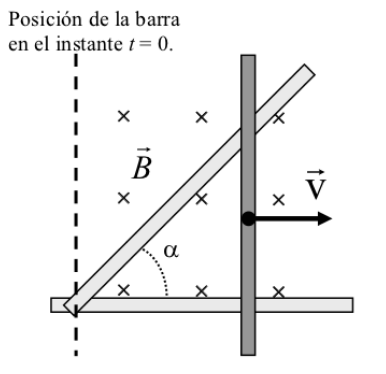
\includegraphics[scale=.45]{cir.png}
\end{minipage}
\vspace{-1.5ex}

\begin{itemize}
				\item[a)]  Calcula la \textbf{fem inducida} en el circuito $15\;s$ después de que la barra empiece a moverse.
				\item[b)] Si la resistencia interna circuito en ese instante es $5\,\Omega$, calcula \textbf{el valor y el sentido} de la corriente inducida en $t=15\;s$. 
			\end{itemize}
\qed
		
\end{enumerate}		
 
\end{document}

